% Author: David Larsen <dcl9934@cs.rit.edu>
% Author: Doug Krofcheck <dpk3062@rit.edu>
\documentclass[11pt]{article}
\usepackage[margin=0.7in]{geometry}
\usepackage{listings}   %
\usepackage{needspace}  %
\usepackage{color}      %
\usepackage{ifthen}     % 
\usepackage{graphicx}   %
\usepackage{csc}        %
\usepackage{tikz}       %
\usetikzlibrary{shapes, arrows, automata} %
\usepackage{tabularx}   % for helping matchtabular (matching questions)
\usepackage{textcomp}	% So our quotes in code don't look like shit
\usepackage{longtable}
\usepackage{multicol}
\setlength{\columnsep}{12em}

\lstset{ %
basicstyle=\footnotesize\ttfamily,       % the size of the fonts that are used for the code
numbers=left,                   % where to put the line-numbers
stepnumber=1,                   % the step between two line-numbers. If it's 1 each line will be numbered
numbersep=5pt,                  % how far the line-numbers are from the code
showspaces=false,               % show spaces adding particular underscores
showstringspaces=false,         % underline spaces within strings
tabsize=4,		                % sets default tabsize to 4 spaces
language=Java,
upquote=true,
columns=fixed
}

\ifthenelse{\isundefined{\isAnswerKey}}
{
    \newenvironment{answer}{\large\lstset{basicstyle=\tiny\ttfamily}\color{white} \small{}}{}
}
{
    \newenvironment{answer}{\large\lstset{basicstyle=\large\ttfamily}\color{red} \small{}}{}
}

% ----- Start matchtabular definition -----
\newcounter{matchleft}
\newcounter{matchright}
\newenvironment{matchtabular}{%
  \setcounter{matchleft}{0}%
  \setcounter{matchright}{0}%
  \tabularx{\textwidth}{%
    >{\leavevmode\hbox to 1.5em{\stepcounter{matchleft}\arabic{matchleft}.}}X%
    >{\leavevmode\hbox to 1.5em{\stepcounter{matchright}\alph{matchright})}}X% 
    }%
}{\endtabularx}
% ----- End matchtabular definition -----

\title{CSCI-140 Midterm Review}
\author{Computer Science Community}
\date{\today}

\makeatletter
\let\thetitle\@title
\let\theauthor\@author
\let\thedate\@date
\makeatother

\begin{document}
\header
\begin{enumerate}

	\item In each of the following situations, would it be better to use array-backed storage or a singly linked list?
\begin{enumerate}
	\item Inserting a random number into a sorted list.
	\begin{answer}
	Linked list --- Constant insertion time, whereas an array would necessitate moving all elements after the insertion point.
	\end{answer}
	
	\item Creating a list that will hold all the players in a game.  The game has a max limit on the number of players.
	\begin{answer}
	Array abstraction --- You have a fixed limit, so pre-allocate enough space for them all.
	\end{answer}

	\item Deleting the last element from the list.
	\begin{answer}
	Array abstraction --- Your linked list would have to iterate all the way down, whereas the array structure can simply change its apparent size.
	\end{answer}
			
	\item Deleting from the head end of the list.
	\begin{answer}
	Linked list --- Constant time operation, versus O($n$) for the array-backed container.
	\end{answer}
\end{enumerate}  



\vspace{24pt}
	
	\item Suppose we are talking about the depth-first search (DFS) algorithm. Nodes are added to the data structures in alphabetical order.
\begin{enumerate}
\item What underlying data structure does this algorithm use?

\begin{answer}
A stack.
\end{answer}

\item
Given the following graph, state the DFS traversal order and show the data structure at each step.
Node \texttt{A} is the start node, and \texttt{F} is the destination node.

\begin{minipage}{0.35\textwidth}
\vspace{-136pt}
\begin{answer}
$\leftarrow$ bottom of stack \\
\textbar A \\
\textbar B C \\
\textbar B D E \\
\textbar B D \\
\textbar B F \\
\textbar B \\

The traversal order is ACEDF.
\end{answer}
\end{minipage}
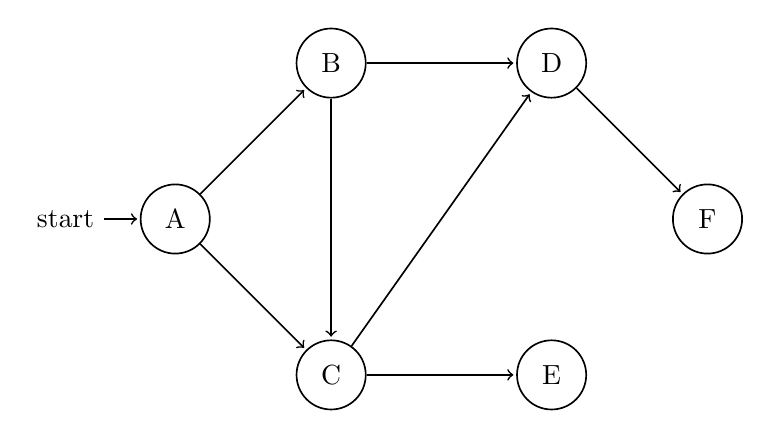
\begin{tikzpicture}[shorten >=1pt,auto,node distance=2.8cm,semithick]
	\node[initial,state] (A) {A};
	\node[state]        (B) [above right of=A] {B};
	\node[state]        (C) [below right of=A] {C};
	\node[state]        (D) [right of=B] {D};
	\node[state]        (E) [right of=C] {E};
	\node[state]        (F) [below right of=D] {F};

	\path[->]   (A) edge node {} (C)
		(A) edge node {} (B)
		(B) edge node {} (C)
		(B) edge node {} (D)
		(C) edge node {} (D)
		(C) edge node {} (E)
		(D) edge node {} (F);
\end{tikzpicture}

\item
What path from \texttt{A} to \texttt{F} does the DFS algorithm return?

\begin{answer}
ACDF 
\end{answer}

\end{enumerate}


	\item Now consider a BFS algorithm, again populating data structures in alphabetical order.
\begin{enumerate}
\item
What changes would need to be made to a DFS implementation to turn it into a breadth-first search (BFS)?

\begin{answer}
Use a queue data structure (instead of a stack).
\end{answer}

\item
Using the graph as described in Question 1, what is the BFS traversal order?
Show the data structure at each step. \\
\begin{answer}
$\leftarrow$ front of queue \\
A \\
B C \\
C D \\
D E \\
E F \\
F \\

The traversal order is ABCDEF.
\end{answer}

\item
What path from \texttt{A} to \texttt{F} results from the BFS algorithm?

\begin{answer}
ABDF
\end{answer}

\end{enumerate}
	
	\item Write code to naturally sort the given list in as few lines as possible. You should not need to write a loop or use any numbers (\texttt{Integer}, \texttt{int}, \texttt{Double}, \texttt{double},
\texttt{BigInteger}, etc...).
\begin{verbatim}
List<String> list = Arrays.asList("a", "o", "d", f", "x");
\end{verbatim}
\begin{answer}
\begin{verbatim}
Collections.sort(list);
//or
TreeSet<String> sorted = new TreeSet<String>(list);
\end{verbatim}
\end{answer}
	
	\item Convert the following code to use generics.
\begin{lstlisting}
interface StringCondition {
	boolean checkString(String s);
}

interface IntegerCondition {
	boolean checkInteger(Integer i);
}

class StringContainer {
	ArrayList<String> values;
	
	// Add and other methods are defined correctly here...

	String getFirstWhereHolds(StringCondition condition) {
		for (String s : values) {
			if (condition.checkString(s))
				return s;
		}
		return null;
	}
}

class IntegerContainer {
	ArrayList<Integer> values;

	// Add and other methods are defined correctly here...

	Integer getFirstWhereHolds(IntegerCondition condition) {
		for (Integer i : values) {
			if (condition.checkInteger(i))
				return i;
		}
		return null;
	}
}
\end{lstlisting}

\begin{answer}
\begin{lstlisting}
interface Condition<E> {
	boolean check(E value);
}

public class Container<E> {
	ArrayList<E> values;
	E getFirstWhereHolds(Condition<E> condition){
		for (E v : values) {
			if (condition.check(v))
				return v;
		}
		return null;
	}
}
\end{lstlisting}
\end{answer}
	
	\item Reimplement the following function using an \texttt{Iterator} instead of a \texttt{for}-each loop.
\begin{lstlisting}[language=java]
public static Integer sum ( ArrayList<Integer> lst ) {
	Integer total = 0 ;
	for( Integer elem : lst ) {
		total = total + elem ;
	}
	return total ;
}
\end{lstlisting}
\begin{answer}
\begin{lstlisting}[language=java]
public static Integer sum (ArrayList<Integer> lst){
	Integer total=0;
	for(Iterator<Integer> iter=lst.iterator();iter.hasNext();){
		Integer cur_val=iter.next(); 
		total=total+cur_val;
	}
	return total;
}
\end{lstlisting}
\end{answer}


\vspace{24pt}

	\item Briefly describe the difference (for objects) between \texttt{a.equals(b)}, \texttt{a==b}, \texttt{a.compareTo(b)},\\ and \texttt{Comparator.compare(a,b)}.

\begin{answer}
\begin{itemize}

\item \texttt{a.equals(b)} Compares objects for equality. 
Class \texttt{Object} provides a default implementation (to be precise, it is \texttt{==} by default) that can be overridden for behavior necessary for a certain class. Returns a \texttt{boolean}.

\item \texttt{a == b}  Checks \textit{memory locations} (if the two objects are the SAME object, as defined by whether or not \texttt{a} and \texttt{b} point to the same spot in memory). Can also be used to check whether \texttt{a} is \texttt{null}. Also returns a \texttt{boolean}.

\item \texttt{a.compareTo(b)} Returns an \texttt{int} indicating whether \texttt{a} is less than (-1),
equal to (0), or greater than (+1) \texttt{b}, according to their natural ordering. Specified by the \texttt{Comparable} interface.

\item \texttt{compare(a,b)} Returns a negative a $<$ b, 0 if a $=$ b, a positive if a $>$ b. \\
With two \texttt{Comparator} objects, \texttt{comp1} and \texttt{comp2},
\texttt{comp1.equals(comp2)} implies that \\ \texttt{sgn(comp1.compare(o1,o2))==sgn(comp2.compare(o1, o2))} for every object reference \texttt{o1} and \texttt{o2}.

\end{itemize}
\end{answer}


	\item Briefly explain the differences between the three kinds of exceptions: checked exceptions, runtime exceptions, and errors.
\begin{answer}

\textbf{checked exceptions} -� Exceptions that a method signature must specify it throws. If a method
may throw a checked exception, all calls to that method must be within a \texttt{try}-\texttt{catch} block. Checked exceptions should be used exclusively for foreseeable runtime mistakes, and any reasonably robust
system should be able to recover from one. Classic example is \texttt{IOException}.\\

\textbf{runtime exception} -� Not declared in a method signature and not anticipated to be thrown.
Usually arise due to software bugs and often cause the program to crash. Classic
examples are \texttt{NullPointerException} and \texttt{ArrayIndexOutOfBoundsException}.\\

\textbf{errors} -� Represent a serious issue outside of the control of the programmer (hard drive
failure, not enough memory, device issue). Examples are \texttt{IOError}, \texttt{VirtualMachineError} and
\texttt{ThreadDeath} (see Java's \texttt{Error} class).
\end{answer}


\vspace{48pt}

	\item Is there anything wrong with the following exception handler as written? Will this
code work as intended? 
\begin{lstlisting}[language=java]
try {
	this.epicFail();
} catch (Exception e) {
	...
} catch (ArithmeticException a) {
	...
}
\end{lstlisting}
\begin{answer}
\texttt{Exception} is more broad than \texttt{ArithmeticException}, so the second \texttt{catch} statement is unreachable.  \texttt{catch} statements should filter possible \texttt{Exception} types from specific to broad.
\end{answer}
	
	\item \textbf{Searching a Graph}
	\begin{enumerate}
		\item
			Write a recursive algorithm that (given a graph, start vertex, and goal vertex),
			determines whether or not there is a path to the goal vertex.

            Assume you are provided with a \texttt{Graph} class with a \texttt{getNeighbors( int vertex )} method, which returns a \texttt{Set\textless Integer\textgreater} representing the numbers corresponding to neighboring vertices. Assume \texttt{visited} is a \texttt{Set} keeping track of all visited vertices. \\
			(Note: Your algorithm should return a Boolean value, not an actual path!)
\begin{verbatim}
boolean hasPathToRec(Graph g, int start, int goal, Set<Integer> visited) {
\end{verbatim}
			
\begin{answer}
\begin{lstlisting}
	if( start == goal ){
		return true;
	} else {
		for( int n : g.getNeighbors(start) ){
			if( ! visited.contains(n) ){
				visited.add(n);
				if ( hasPathToRec(g, n, goal, visited) )
					return true;
			}
		}
		return false;
	}
}
\end{lstlisting}
\end{answer}
		            
		\item
			Rewrite your algorithm to be iterative instead. \\
			(Hint: What data structure do you need to use if you no longer have recursion?)
\begin{verbatim}
boolean hasPathToIter(Graph g, int start, int goal, Set<Integer> visited) {
\end{verbatim}	
			
\begin{answer}
\begin{lstlisting}
	Stack<Integer> theStack = new Stack<Integer>();
	theStack.push(start);
	visited.add(start);
	while( ! theStack.empty() ){
		int curr = theStack.pop();
		if( curr == goal ){
			return true;
		}
		for( int n : g.getNeighbors(curr) ){
			if( ! visited.contains(n) ) {
				visited.add(n);
				theStack.push(n);
			}
		}
	}
	return false;
}
\end{lstlisting}
\end{answer}
	\end{enumerate}

	
	\item %
% NOTE: This question is meant to take up one full page
%	and includes all necessary spacing.
%


Show the stages of a merge sort and a quicksort on the following list:
      [3,5,1,3,2,7,9]. Be sure to identify your pivot.

    \begin{answer}
	merge sort:\\*
	\newline
    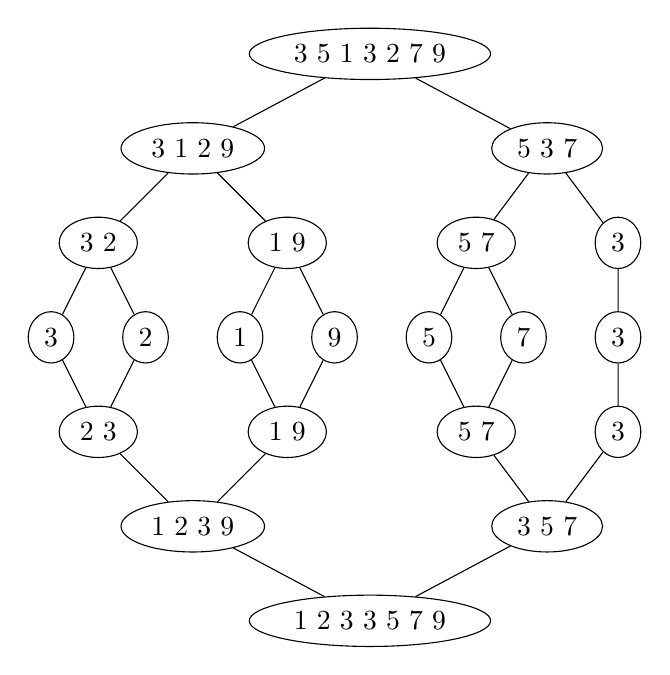
\begin{tikzpicture}[scale=1.2]
	\node [draw,ellipse] at (3.375,3) (head) {3 5 1 3 2 7 9};
	\node [draw,ellipse] at (1.5,2) (1) {3 1 2 9};
	\node [draw,ellipse] at (5.25,2) (2) {5 3 7};
	\node [draw,ellipse] at (.5,1) (3) {3 2};
	\node [draw,ellipse] at (2.5,1) (4) {1 9};
	\node [draw,ellipse] at (4.5,1) (5) {5 7};
	\node [draw,ellipse] at (6,1) (6) {3};
	\node [draw,ellipse] at (0,0) (7) {3};
	\node [draw,ellipse] at (1,0) (8) {2};
	\node [draw,ellipse] at (2,0) (9) {1};
	\node [draw,ellipse] at (3,0) (10) {9};
	\node [draw,ellipse] at (4,0) (11) {5};
	\node [draw,ellipse] at (5,0) (12) {7};
	\node [draw,ellipse] at (6,0) (13) {3};
	\node [draw,ellipse] at (.5,-1) (14) {2 3};
	\node [draw,ellipse] at (2.5,-1) (15) {1 9};
	\node [draw,ellipse] at (4.5,-1) (16) {5 7};
	\node [draw,ellipse] at (6,-1) (17) {3};
	\node [draw,ellipse] at (1.5, -2) (18) {1 2 3 9};
	\node [draw,ellipse] at (5.25, -2) (19) {3 5 7};
	\node [draw,ellipse] at (3.375,-3) (20) {1 2 3 3 5 7 9};

	\path [draw] (1) -- (head) -- (2);
	\path [draw] (3) -- (1) -- (4);
	\path [draw] (5) -- (2) -- (6);
	\path [draw] (7) -- (3) -- (8);
	\path [draw] (9) -- (4) -- (10);
	\path [draw] (11) -- (5) -- (12);
	\path [draw] (13) -- (6);
	\path [draw] (7) -- (14) -- (8);
	\path [draw] (9) -- (15) -- (10);
	\path [draw] (11) -- (16) -- (12);
	\path [draw] (13) -- (17);
	\path [draw] (14) -- (18) -- (15);
	\path [draw] (16) -- (19) -- (17);
	\path [draw] (18) -- (20) -- (19);
	\end{tikzpicture}\\*
	\newline
	Quicksort (using the first element in the list as a pivot):\\*
	\newline
	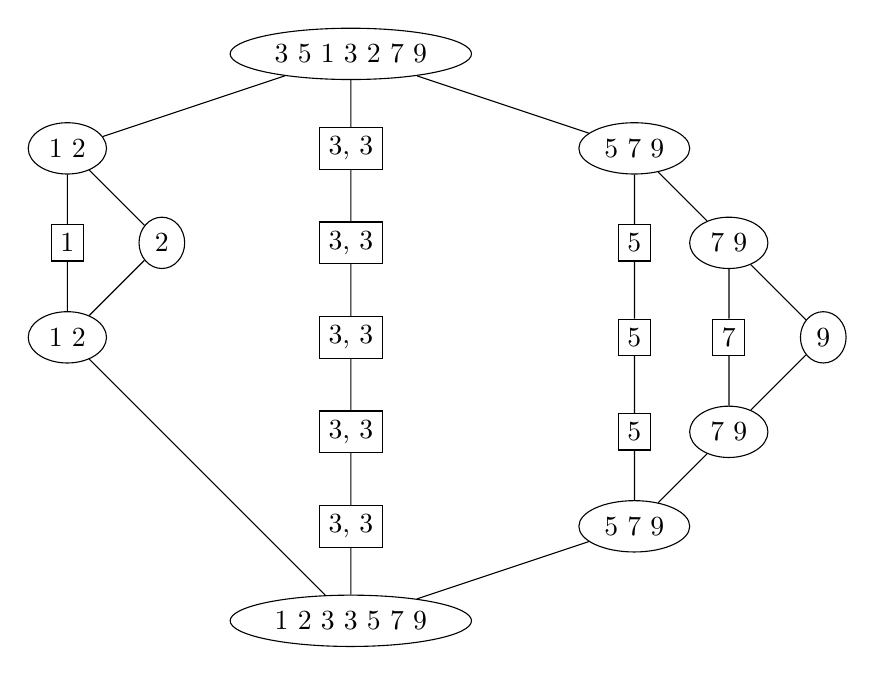
\begin{tikzpicture}[scale=1.2]
	\node [draw] at (4,0) (4) {3, 3};
	\node [draw] at (7,0) (5) {5};
	\node [draw] at (8,0) (6) {7};
	\node [draw,ellipse] at (9,0) (7) {9};
	\node [draw] at (1,1) (8) {1};
	\node [draw, ellipse] at (2,1) (9) {2};
	\node [draw] at (4,1) (10) {3, 3};
	\node [draw] at (7,1) (11) {5};
	\node [draw,ellipse] at (8,1) (12) {7 9};
	\node [draw, ellipse] at (1,2) (13) {1 2};
	\node [draw] at (4,2) (14) {3, 3};
	\node [draw,ellipse] at (7,2) (15) {5 7 9};
	\node [draw,ellipse] at (4,3) (16) {3 5 1 3 2 7 9};
	\node [draw] at (4, -1) (19) {3, 3};
	\node [draw] at (7,-1) (20) {5};
	\node [draw, ellipse] at (8,-1) (21) {7 9};
	\node [draw, ellipse] at (1,0) (22) {1 2};
	\node [draw] at (4,-2) (23) {3, 3};
	\node [draw, ellipse] at (7,-2) (24) {5 7 9};
	\node [draw, ellipse] at (4,-3) (25) {1 2 3 3 5 7 9};

	\path [draw] (8) -- (13);
	\path [draw] (8) -- (22);
	\path [draw] (9) -- (22);
	\path [draw] (9) -- (13);
	\path [draw] (4) -- (10) -- (14) -- (16);
	\path [draw] (5) -- (11) -- (15);
	\path [draw] (6) -- (12);
	\path [draw] (7) -- (12) -- (15) -- (16);
	\path [draw] (13) -- (16);

	\path [draw] (22) -- (25);
	\path [draw] (4) -- (19) -- (23) -- (25);
	\path [draw] (5) -- (20) -- (24);
	\path [draw] (6) -- (21);
	\path [draw] (7) -- (21) -- (24) -- (25);

	\end{tikzpicture}
    \end{answer}

	\item ../../141/questions/sorting_run_times.tex

	\item ../../141/questions/quicksort_worst_case_when.tex

	\item What causes Quicksort to run so slowly on the input you describe in question \ref{qsort-worst-case}?

    \begin{answer}
    Quicksort splits its input into two lists based on the value of the pivot.
    If the pivot is either the smallest or the largest element, then one list
    will only have no elements, while the others will have all of the elements
    but the pivot. We can see this if we perform a substitution trace:
\begin{verbatim}
qsort([1,2,3,4])
qsort([]) + [1] + qsort([2,3,4])
qsort([]) + [1] + qsort([]) + [2] + qsort([3,4])
qsort([]) + [1] + qsort([]) + [2] + qsort([]) + [3] + qsort([4])
qsort([]) + [1] + qsort([]) + [2] + qsort([]) + [3] + qsort([4])
qsort([]) + [1] + qsort([]) + [2] + qsort([]) + [3] + qsort([]) + [4] + qsort([])
[1,2,3,4]
\end{verbatim}
    \end{answer}

	\itemSuppose you have an encoded file called secret.txt that must be decoded using a stream called DecodeStream.  
Write code to read the file, decode it using the DecodeStream, and print the contents.  
Assume the containing method throws all IOExceptions and DecodeStream is implemented to correctly handle buffered input.

\begin{answer}
\begin{lstlisting}[language=java]
String line;
DecodeStream in = new DecodeStream( new BufferedReader( 
new FileReader( "secret.txt" ) ) );
while( ( line = in.readLine() ) != null ) {
	System.out.println( line );
}
\end{lstlisting}
\end{answer}

\vspace{24pt}


\end{enumerate}
\end{document}

